\chapter{Modelo do trabalho}

    Neste capítulo será definido como será feita a coleção dos dados, quais serão os tipos de dados que serão coletados e qual será o tipo de aplicação da mineração de uso que sera utilizada.

    Os usuários da internet estão deixando rastros a todo momento enquanto navegam pela web, esses rastros são as informações que serão coletadas para serem processadas e analisadas para a geração dos perfis de usuários e padrões de uso.

    Para que o objetivo deste trabalho seja alcançado, é necessário que seja feito um estudo para que a escolha de quais serãos as informações que deverão ser retiradas dos rastros deixados pelo usuário, pois dependendo da necessidade, deve ser utilizada um tipo de informação diferente e para que os perfis coletados tenham uma certa riqueza de informações para que seja possível fazer uma boa análise de perfis, é preciso que a coleta seja feitas com foco nos rastros corretos.

\begin{figure}[!htb]
\centering
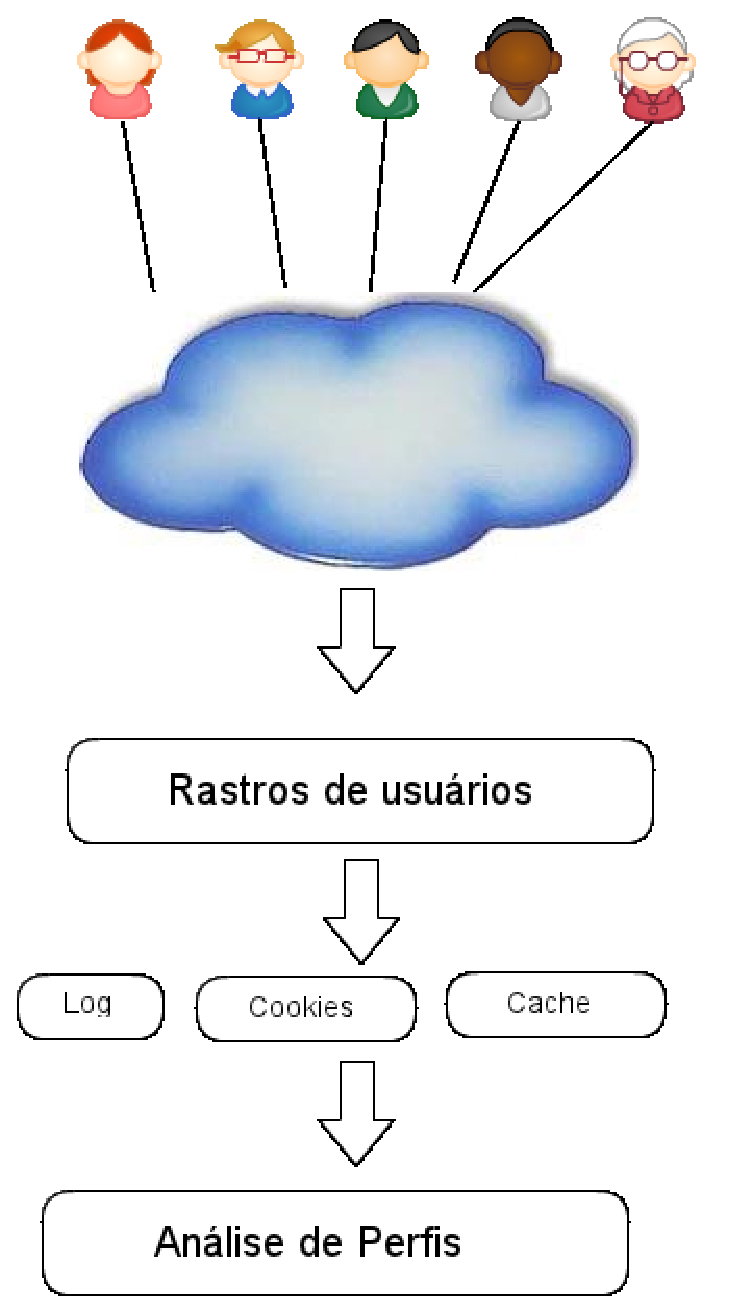
\includegraphics[scale=0.7]{diagrama}
\caption{Fluxo de informações dos usuários}
\label{Rotulo}
\end{figure}

